\documentclass{article}
\usepackage{subcaption}
\usepackage{caption}
\usepackage{xcolor}
\usepackage[margin=1in]{geometry} % 设置页边距为1英寸,您可以根据需要更改
% if you need to pass options to natbib, use, e.g.:
% \PassOptionsToPackage{numbers, compress}{natbib}
% before loading nips_2016
%
% To avoid loading the natbib package, add option nonatbib:
% \usepackage[nonatbib]{nips_2016}
\usepackage{svg}
\PassOptionsToPackage{numbers,sort&compress}{natbib}
\usepackage[final]{nips_2016} % produce camera-ready copy
\usepackage{graphicx}
\usepackage[utf8]{inputenc} % allow utf-8 input
\usepackage[T1]{fontenc}    % use 8-bit T1 fonts
\usepackage{hyperref}       % hyperlinks
\usepackage{url}            % simple URL typesetting
\usepackage{booktabs}       % professional-quality tables
\usepackage{amsfonts}       % blackboard math symbols
\usepackage{nicefrac}       % compact symbols for 1/2, etc.
\usepackage{microtype}      % microtypography

\title{Spotify Music Popularity Prediction}

% The \author macro works with any number of authors. There are two
% commands used to separate the names and addresses of multiple
% authors: \And and \AND.
%
% Using \And between authors leaves it to LaTeX to determine where to
% break the lines. Using \AND forces a line break at that point. So,
% if LaTeX puts 3 of 4 authors names on the first line, and the last
% on the second line, try using \AND instead of \And before the third
% author name.

\author{
  S2441797\\
  %% examples of more authors
  \And
  S2500272\\
 \And
  S2530615\\
}

% 表格前调整行间距
\renewcommand{\arraystretch}{0.4}

\begin{document}

\maketitle

\begin{abstract}
The focus of this report is on the task of predicting whether songs will become popular within a specified number of days in the future. We focus on data exploration, simply and efficiently handling intrinsic time issues without explicitly using time models, and improving classification task performance by using multiple classifiers. We evaluated all models and selected CatBoost (AUC = 0.968) as the best classification algorithm. We further explored the influence of various feature types and the optimization of hyperparameters in the model.
\end{abstract}

\section{Introduction}
Spotify is the world's largest streaming service provider, with over 205 million subscribers as of the end of 2022\cite{usercounts}. Given Spotify's large audience, its daily rankings have become a very authoritative reference for measuring whether music is popular enough. We believe that artists are very interested in knowing if and when their works will become popular on this platform.

Predicting music trends is of great benefit to record companies and artists. For example, developing market strategies based on predicted results can help investors and music industry-related companies make wiser investment and cooperation decisions by understanding which songs may become popular.

The prediction of song popularity has received much attention in recent years, and three main approaches are currently used. First, the popularity potential of new songs can be predicted by analyzing the acoustic properties of previously popular songs \cite{8327835}. Second, methods for predicting song popularity in response to the analysis of social media data; these methods have been widely explored in the scientific literature \cite{shulman2016predictability}. The third is an approach that we expect to explore and expand upon, which is the use of historical song ranking data from every day in the past to predict whether a song will be popular in the future \cite{8999039}. In this report, we define popular songs as those that appear in Spotify's "Top 50" charts, which is similar to defining popularity in terms of yearly rankings \cite{881888}.

\section{Exploratory data analysis}
The dataset contains 20 field information for all 651936 tracks (with 'id' as the main key) that were listed on the Spotify 'TOP200' chart from January 1, 2017, to May 31, 2023, totalling 9151 songs. It can be divided into three categories: 7 acoustic features about the music track itself, 4 artist-related features, including artist name, continent, country, and artist points on this song, as well as time characteristics. The release date of the ranking list. In addition, in order to explore the relationship between song popularity and the length of time the song has been on the market, we also used Spotify's web API to capture the release date of each song and processed it as the difference from the 'Date' tag representing the release date of the song chart, named 'Time gap'

Acoustic features include 'Danceability', 'Energy', 'Speediness', 'Acousticness', 'Instrumentalness', 'Valence', and 'Loudness'. Due to the significant range of data for 'Loudness', we have normalized it (\autoref{fig:boxplot}). We believe that the seasonal trend of the vocal features of the song is not significant, and the 'Danceability' feature with the largest data span has a range of no more than 0.1 (\autoref{fig:feature_trends}). There is no significant difference in the acoustic feature distribution between songs that have ranked on the top 50 at least once and songs that have never appeared before\autoref{fig: distribute}

The 'Top 200' ranking released by Spotify attempts to summarize the statistical data of the most popular songs on a daily basis, in order to generate the popularity ranking of songs. Therefore, the ranking of songs in the chart is basically a time-domain signal, representing their popularity over time. A debute point is defined as the first ranking of a song on the chart. Most songs have a lower ranking when they first appear on the chart, with 17.53\% of songs entering the top 50 on the first chart, and a few songs debuting with the highest ranking (less than 0.4\%)\autoref{fig:debut}.

By drawing the length of the time span (in weeks) of songs on the charts for each year, we found that this span presents a trend distribution that can be found\autoref{fig:length}. About 19.81\% of the data on the charts spans no more than one week, and 37.76\% of the data spans over 48 weeks. With such a trendy time span, It is possible to effectively predict the future trend of song popularity by adding time-related features.

Analysing the Autocorrelation Function (ACF) and Partial Autocorrelation Function (PACF) of the time series data \autoref{fig:acf}\autoref{fig:pacf}, it is observed that the song rankings show significant short-term autocorrelation. This suggests that past observations have a significant effect on future values only in a short time frame. The rapid decay in the ACF graphs, as well as the significant drop in the PACF graphs after the number of lagged features $k=1$, jointly suggests that the data exhibits first-order monotonicity. Based on these observations, the data are best suited for the application of a first-order autoregressive model (AR(1) model), which is judged to be optimal for relying only on observations with the number of lagged features $k=1$.

\begin{figure}[ht]
  \centering
  \begin{subfigure}[t]{0.45\textwidth}
    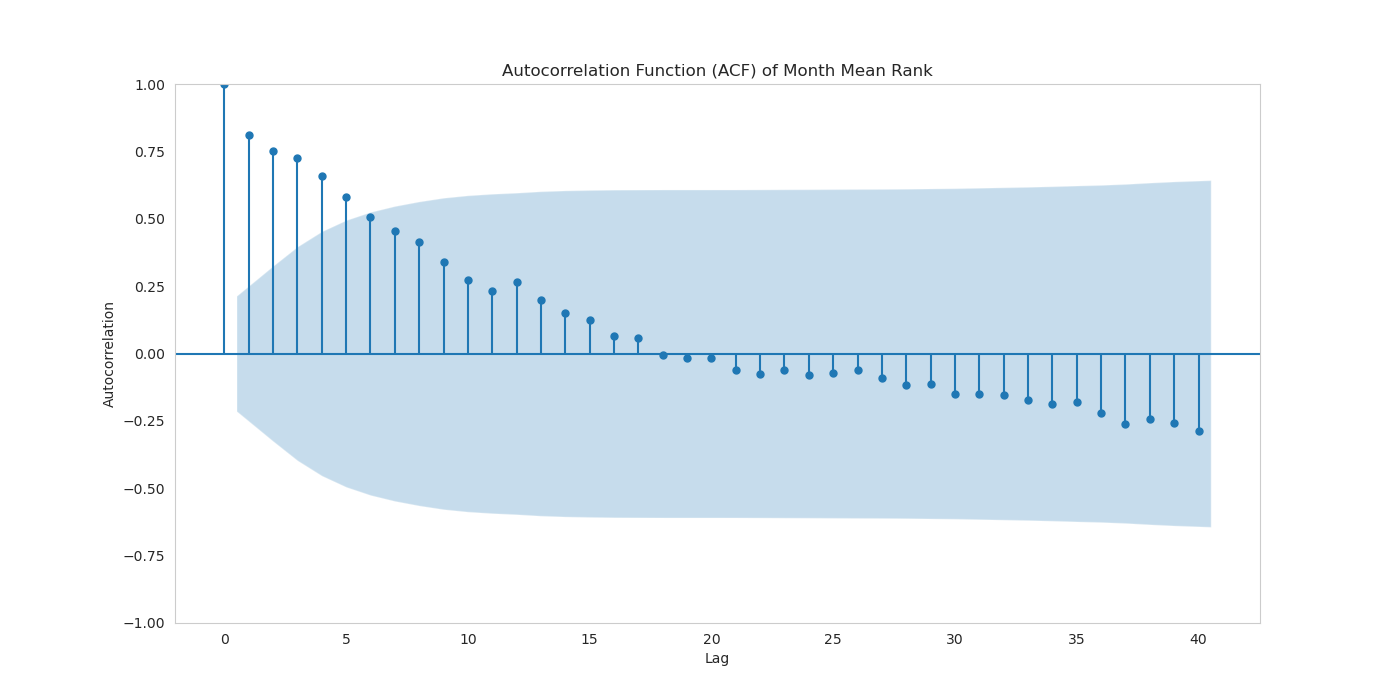
\includegraphics[width=\textwidth]{acf.png}
    \captionsetup{labelformat=default}
    \caption{Autocoorelation Function(ACF) of Month Mean Rank.The blue-shaded area represents the level of significance. According to the ACF chart, it can be concluded that the data shows a certain time dependence, especially in the short-term lag period.}
    \label{fig:acf}
  \end{subfigure}
  \hfill
  \begin{subfigure}[t]{0.45\textwidth}
    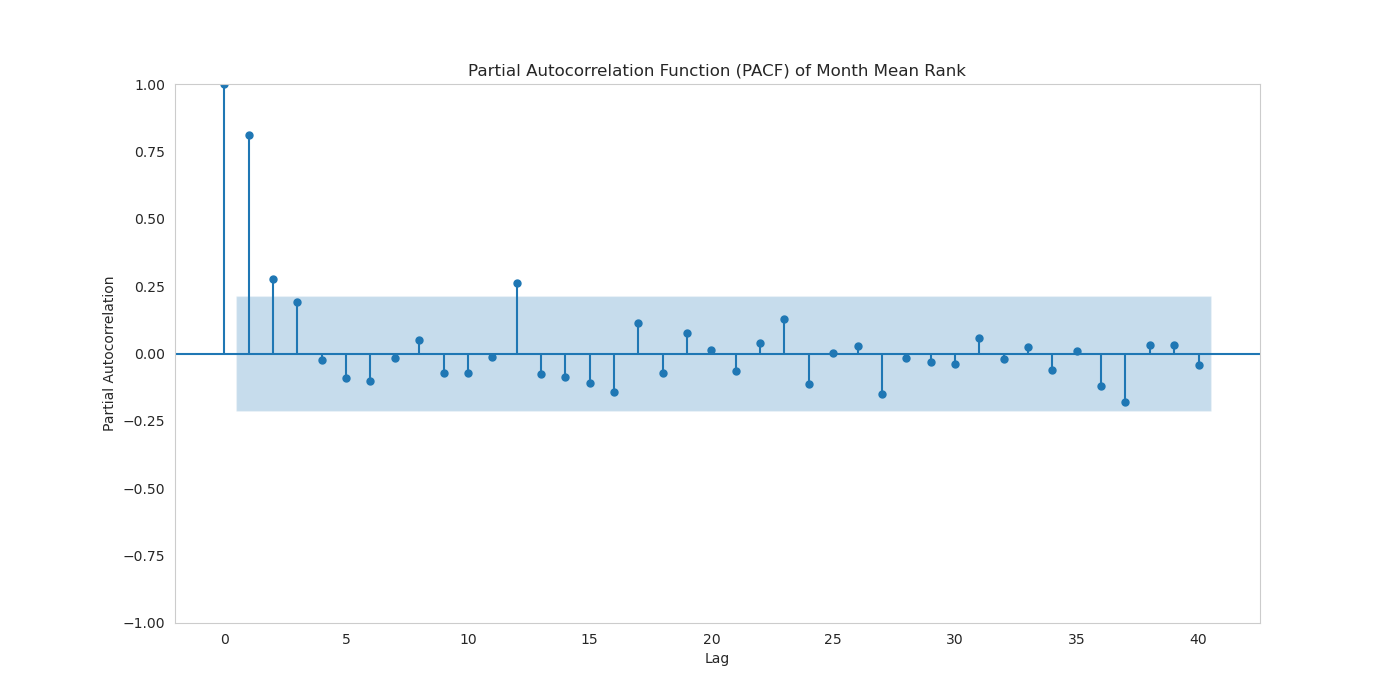
\includegraphics[width=\textwidth]{pacf.png}
    \captionsetup{labelformat=default}
    \caption{Partial Autocorrelation Function (PACF) of Month Mean Rank. It shows the correlation of the time series with itself at the lags after removing the effect of the intermediate lag terms. As can be seen from the figure, after controlling for the effects of the other lags, the first few lags, especially the first one, still have a direct and significant effect on the current value.}
    \label{fig:pacf}
  \end{subfigure}
  \caption{Autocorrelation analysis of time series features}
  \label{aat}
\end{figure}
\section{Data preprocessing}
The completeness and reasonableness of the dataset were tested and found that there were no missing values in the data. According to the definition of LUFS, the unit of Spotify's 'Loudenss', its maximum value is 0 \cite{lloudness}, so the four songs containing outliers with 'Loudness' greater than 0 were removed from our dataset. Also, the loudness extreme difference is large, so we normalised it. And 'Instrumentalness' was binaryised.

Song popularity may be correlated with the Artist's own success, which can be defined in a variety of ways; one way to add an artist popularity feature is to define a 'Superstar' label\cite{Interiano2018MusicalTA}, where an artist is said to be a 'Superstar' if his or her work has been ranked Top 10 at least once during the period of the dataset's collection. We also one-hot encoded the 'Continent' feature.

We also attempted to quantify the degree of popularity of artists by accumulating 'Points (Ind for each Artist/Nat)', where higher scores imply greater fame of the artist.

Define $U$ to be the set of all songs during the dataset collection period, and $Pi$ to be the set of songs that appeared at least once on the 'Top50' chart for the ith time interval. For the daily charts, we can generate 200 instances of each song $s_{i,j} \in U$ converted into a feature vector $xi,j$. We assign each instance with a feature - popularity. This binary variable indicates whether the song was popular during that time interval.

Subsequently, we use lagged features to transform complex correlations into linear relationships that are easier to model. This means that the introduction of lagged features allows us to use known historical data to predict future values without relying on a specific time model. Let $Xi = {xi,1, xi,2, ... , xi, |U|}$ be the set of instances for a specific time interval. Then by, adding $xi+\delta,j, xi+2\delta,j, ... , xi+k\delta,j$ to the lag feature to enhance the instances\cite{8999039}. Lagged features are binary variables that indicate the popularity of a song in the $i-k$th time interval, i.e., $k*\delta$ days ago. The number of lagged features is set $k = 1$ based on previous analyses.

Add the feature 'Target' that indicates whether the song is popular in the $i+1$th time interval, i.e., $\delta$ days later. Our method requires that $\delta$ and $k$ be kept constant in the training set and the application set.

The final step in constructing the dataset consists of converting non-numeric features. We replaced 'Date' as well as 'Time gap' with epochs and removed features 'Title', 'Artists', '\# of Artist', 'Artist (Ind.)', 'Points (Ind for each Artist/Nat)', 'Song URL', ' Nationality', '\# of Nationality'.

The Pearson correlation coefficient is a key statistical tool when quantifying linear associations between musical properties. Danceability is moderately positively correlated with Valence ($r=0.40$)\autoref{fig:heatmap}, indicating that tracks with higher melodic pleasure tend to be more danceable. Conversely, Acousticness showed a moderately negative correlation with Energy ($r=-0.54$), revealing that acoustic tracks tend to have lower energy levels. There was a strong positive correlation (r=0.78) between lagging characteristics ('Popularity\_Lag\_1') and current popularity (Popularity), demonstrating the persistence of song popularity. In addition, a moderate positive correlation ($r=0.33$) between an artist's star status ('Superstar') and song popularity implies that works by well-known artists tend to be more popular. The negative correlation of the 'time\_gap' with the target variable may reflect the relationship between the proximity of a song's release and its increase in popularity.

\begin{figure}[h]
  \centering
  \includesvg[width=0.6\textwidth]{heatmap}
  \captionsetup{labelformat=default}
  \caption{Features correlation Heatmap. The color block indicates the correlation between the horizontal and vertical labels, with darker blue indicating a higher degree of negative correlation and darker red indicating a higher degree of positive correlation}
  \label{fig:heatmap}
\end{figure}

\section{Methodology}
In this section, we describe how we constructed cross-validation suitable for unique data found what we consider to be the most appropriate classifiers, and cross-validated each of these classifiers to assess their generalisation ability.

In tackling the supervised learning task on a dataset with multiple features, considerations include the dataset's substantial size, featuring 31 attributes of both numerical and categorical types. To balance predictive accuracy and mitigate overfitting in this scenario, diverse models such as RandomForest, Naive Bayes, CART Decision Tree, Logistic Regression, XGBoost, and CatBoost are explored. The choice between these models takes into account the dataset's linearity, with simpler models like Logistic Regression suitable for linear relationships, while ensemble methods such as RandomForest and XGBoost offer versatility for capturing complex patterns. The computational efficiency of training large datasets is a crucial factor, favoring models like Logistic Regression alongside sophisticated algorithms like XGBoost and CatBoost.


\subsection{Classification Models}
The prediction purpose of our classification task is to determine whether the song will be popular or not in the coming period. Based on two common classification models: plain Bayes and decision tree, we extend the decision tree by choosing two more complex integrated models, XGBoost and CatBoost, which have been used in related studies to achieve good classification results\cite{appxgboost}.

We chose simpler probabilistic models from Plain Bayes, which can be trained more quickly, as well as logistic regression, and used decision tree algorithms as a comparison to complex decision tree models, as well as integrated models XGBoost, CatBoost and Random Forests\cite{rf}.

Random forest is a classification tree-based prediction method compared to classification tree methods that rely on a single tree, it overcomes overfitting by combining the predictions from a list of decision trees, the method not only improves the generalization ability of a single decision tree but also balances the error well in datasets with uneven category representation.

CatBoost was chosen to effectively handle datasets with unbalanced categories and has a variety of built-in techniques for preventing overfitting, which is especially important in areas such as music popularity prediction, where both XGBoost and CatBoost have good mechanisms for handling different types of data features\cite{xgboost}\cite{catboost}.

\subsection{Training and prediction}
For our similar time series processing, we use the ExpandingWindowSplitter\autoref{fig:ExpandingWindowSplitter} to implement a cross-validation approach that considers the temporal dependence of the time series data. This approach ensures that the data in the training set always comes before the test set. By calculating a series of scores, we assess the generalisation ability of our model.

We define the dataset to contain a total number of days $T$. For the $i$th round of experiments, we chose the ranking data with Start date = 1 February 2017 and End date = Start date + $(i-1)*T/6$ as the base date for the training dataset\autoref{fig:ExpandingWindowSplitter}. The days from End date + $T$ to End date + $(1/6)*T$ are allocated as the base date for the test set.

\begin{figure}[h] % 可以使用figure环境来控制图片的浮动位置,选项[h]表示将图片放在当前位置
  \centering
  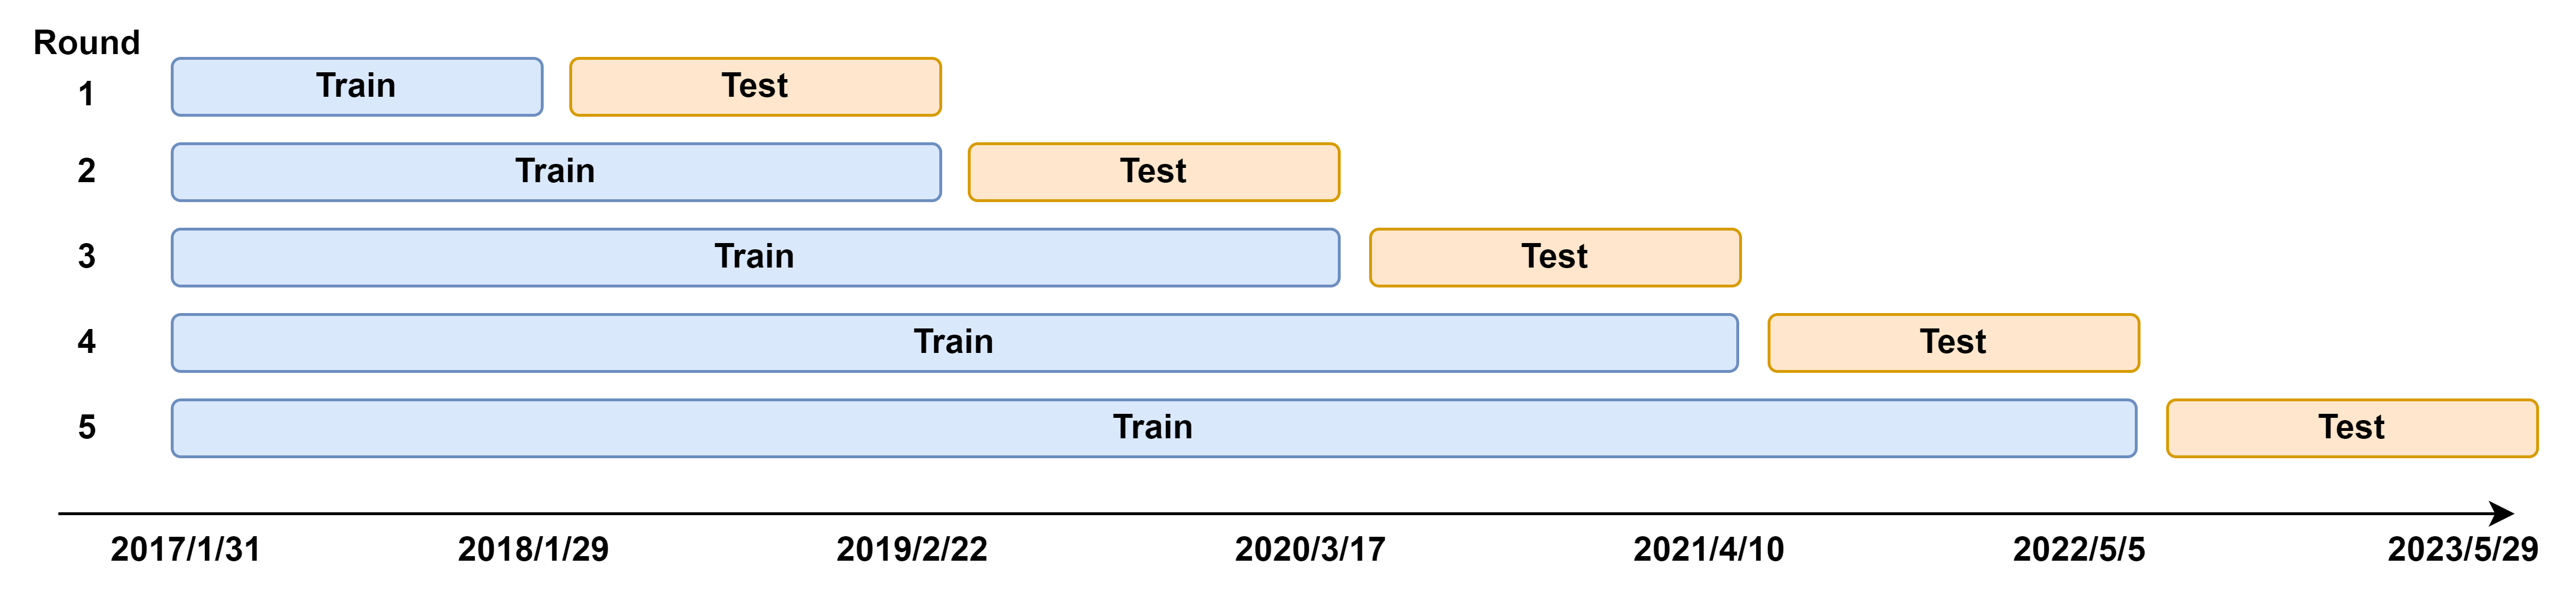
\includegraphics[width=0.7\textwidth]{kfold.drawio.png}
  \captionsetup{labelformat=default}
  \caption{ExpandingWindowSplitter. It generates folds on a sliding window over time, and the length of the training sequence grows over time, with each subsequent fold retaining a full sequence history. The length of the test sequence is constant for each fold.}
  \label{fig:ExpandingWindowSplitter}
\end{figure}

These data have a lag characteristic with a lag period $\delta = 30$ days and quantity $k = 1$ \autoref{fig:lag}. We then use a classifier to predict the popularity of each song 30 days after the base date. The model can only predict 30 days after the base date. For example, assuming the base date is 28 February 2018, it needs to carry lagged features for 29 January 2018 and it can predict the popularity of songs on 30 March 2018. Actually, it is possible to make predictions for earlier points in time through multiple rounds of generalisation and prediction. In this process, characteristics from the preceding prediction round are utilised as features for the current round.

\begin{figure}[h] % 可以使用figure环境来控制图片的浮动位置,选项[h]表示将图片放在当前位置
  \centering
  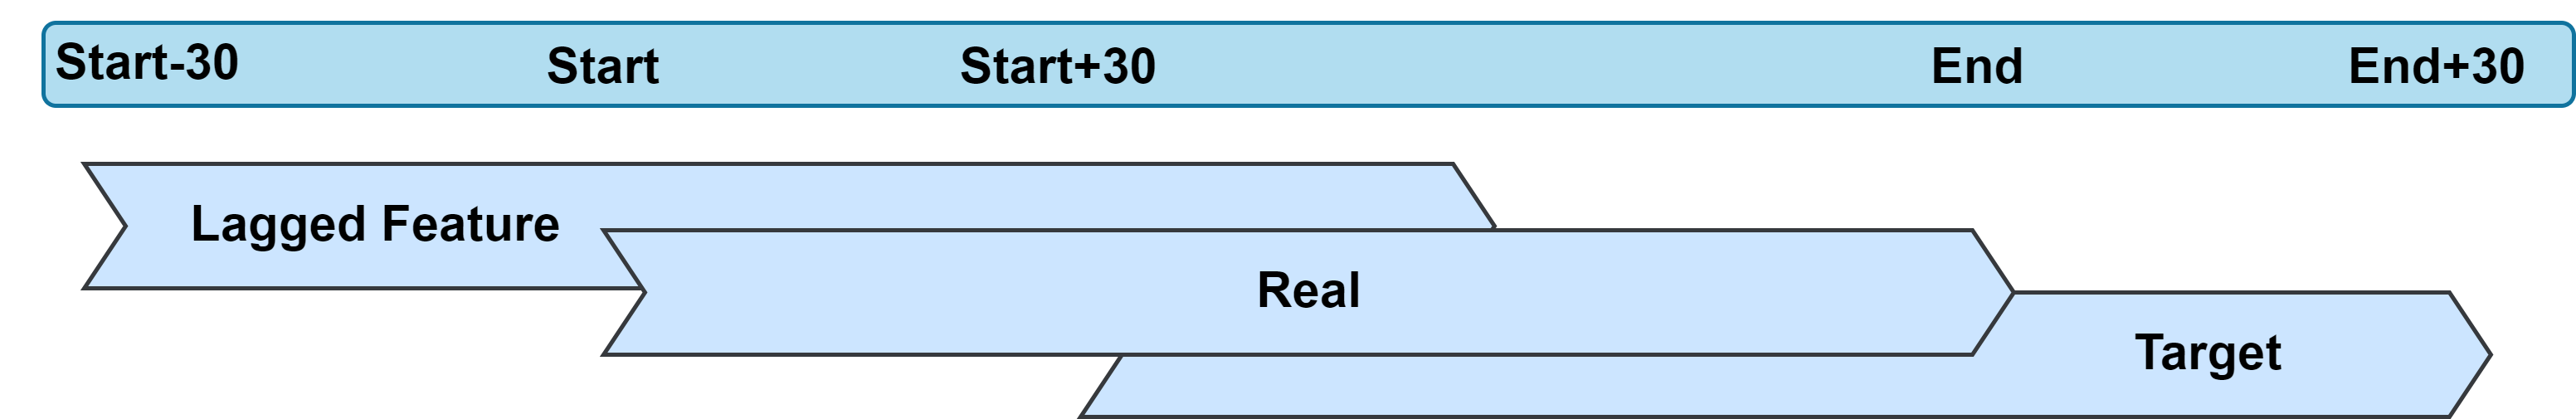
\includegraphics[width=0.7\textwidth]{lag.drawio.png}
  \captionsetup{labelformat=default}
  \caption{Description of the composition of the dataset. 'Start' represents the date on which the base date begins and 'End' represents the date on which the base date ends. Each instance takes with it a lagged feature representing data from thirty days ago and makes a prediction for data from thirty days later.}
  \label{fig:lag}
\end{figure}

\subsection{Hyperparameter Optimisation}
Because tuning machine learning hyperparameters can make the model perform best in a specific task improve model performance, prevent overfitting and accelerate convergence \cite{hyper}. Therefore we tried different combinations of hyperparameters for tuning.
In several of our classifiers, for integrated methods such as Random Forest, the balance between the number of trees (n\_estimators) and the maximum depth of each tree directly affects the performance of the model\cite{hyperbook}. In the field of gradient boosting frameworks represented by XGBoost and CatBoost, key hyperparameters include the learning rate, the number of estimators, and the depth of the trees. In order to improve the simplicity and effectiveness of logistic regression, the hyperparameters mainly revolve around the regularization strength (C) and the type of penalty (L1 or L2). These parameters control the complexity of the model through the size of the penalty coefficients, thus effectively preventing overfitting. We perform the optimization of hyperparameters by grid search.

\section{Results}

\begin{table}[ht]
\centering
\caption{Results of Models}
\label{tab:withacoustics}
\begin{tabular}{p{1.2cm}p{1cm}p{1cm}p{1cm}p{1.2cm}p{1cm}p{1.2cm}p{1cm}}
\toprule
& XG\newline Boost & Random\newline Forest & Naive Bayes & Logistic\newline Regression & Cat\newline Boost & CART\newline D-tree & SVC\newline (RBF)\\
\midrule
Accuracy              & 0.908 & 0.904 & 0.894 & 0.904 & \textcolor{red}{0.920} & 0.831 & 0.908 \\
AUC                   & 0.961 & 0.958 & 0.930 & 0.951 & \textcolor{red}{0.964} & 0.840 & 0.944 \\
F1       & 0.908 & 0.905 & 0.889 & 0.903 & \textcolor{red}{0.919} & 0.835 & 0.898 \\
Precision & 0.909 & 0.907 & 0.902 & 0.906 & \textcolor{red}{0.921} & 0.850 & 0.901 \\
Recall   & 0.908 & 0.904 & 0.894 & 0.904 & \textcolor{red}{0.920} & 0.831 & 0.897 \\
\bottomrule
\end{tabular}
\end{table}
% 表格结束

\begin{table}[ht]
\centering
\caption{Results of Models without Acoustic Features}
\label{tab:model_withoutacoustic}
\begin{tabular}{p{1.2cm}p{1cm}p{1cm}p{1cm}p{1.4cm}p{1cm}p{1.2cm}}
\toprule
& XG\newline Boost & Random\newline Forest & Naive Bayes & Logistic\newline Regression & \ Cat\newline Boost & CART D-Tree \\
\midrule
Accuracy              & 0.907 & 0.908 & 0.894 & 0.904 & \textcolor{red}{0.914} & 0.847 \\
AUC                   & 0.961 & 0.958 & 0.931 & 0.951 & \textcolor{red}{0.961} & 0.845 \\
F1 & 0.907 & 0.908 & 0.889 & 0.903 & \textcolor{red}{0.913} & 0.849 \\
Precision& 0.910 & 0.910 & 0.903 & 0.906 & \textcolor{red}{0.917} & 0.858 \\
Recall   & 0.907 & 0.908 & 0.894 & 0.904 & \textcolor{red}{0.914} & 0.847 \\
\bottomrule
\end{tabular}
\end{table}

\begin{table}[ht]
\centering
\caption{Results of Models without Artist Features}
\label{tab:without artist}
\begin{tabular}{p{1.2cm}p{1cm}p{1cm}p{1cm}p{1.2cm}p{1cm}p{1.2cm}}
\toprule
& XG\newline Boost & Random\newline Forest & Naive Bayes & Logistic\newline Regression & Cat\newline Boost & CART D-Tree \\
\midrule
Accuracy              & 0.804 & 0.798 & \textcolor{red}{0.891} & 0.891 & \textcolor{red}{0.844} & 0.741 \\
AUC                   & 0.916 & \textcolor{red}{0.918} & 0.906 & 0.908 & 0.915 & 0.769 \\
F1 & 0.808 & 0.803 & 0.886 & \textcolor{red}{0.886} & 0.846 & 0.749 \\
Precision& 0.836 & 0.835 & 0.899 & 0.898 & \textcolor{red}{0.857} & 0.797 \\
Recall   & 0.804 & 0.798 & \textcolor{red}{0.891} & 0.891 &  0.844 & 0.741 \\
\bottomrule
\end{tabular}
\end{table}


\section{Discussion}
In this section, we evaluate the effectiveness of different machine learning models for predicting whether future songs will be popular in the next month. Because our dataset is unbalanced (about 2:1), accuracy alone is not a good measure of model performance. We pick multiple metrics that are more robust to imbalance to evaluate our model, and we focus on the values of recall, F1 score, and AUC used to capture how well our model performs in the classification task. Precision measures the fraction of samples that are classified as really popular, while recall measures the fraction of really popular samples that our model classifies as popular. The F1 score serves as a weighted average between these two values. The AUC represents the probability that the classifier ranks a random positive example higher than a random negative one. 

The results presented in \autoref{tab:withacoustics} indicate that the CatBoost model outperformed other models on evaluation metrics including AUC, F1 score, Precision, and Recall, achieving scores of 0.964, 0.919, 0.921 and 0.920 respectively. These suggest that CatBoost is highly effective in accurately classifying songs into popular and not popular categories. The CART decision tree classifier was the lowest performing of all the treatments with an AUC value of 0.840. Comparing Random Forest and XGBoost, both perform very similarly on the test set and both are higher than a single decision tree, suggesting that integrated learning improves the prediction of the model.

Support vector machines must calculate a decision boundary or separating hyperplane that maximises the distance from any class's closest point to the decision boundary to create an optimal boundary classifier. In high-dimensional spaces, identifying these support vectors may call for more computational resources. We did not cross-validate all datasets in our further exploration due to our limited computational resources, and SVM was not the most efficient model for us.

On the other hand, the best model in our study did not show significant performance gains when using acoustic features in  \autoref{tab:model_withoutacoustic}. The performance of the CatBoost classifier with artist features is only 5.3\% higher than that of the CatBoost Classifier without artist features, \autoref{tab:withacoustics}, \autoref{tab:without artist}. This indicates that artists' features did not have a significant impact on our performance in our experiments, and they may not be necessary to achieve satisfactory results.



\section{Conclusions}
For our binary classification problem, our models succeed in achieving good performance through XGBoost and CatBoost. The models predict whether a song will appear in the top 50 of Spotify's global charts 30 days after the base date with over 90\% accuracy, recall, F1 and AUC values.

For further work, we believe that the feature capture in the data can be refined by introducing more sophisticated time series models such as Convolutional Neural Networks (CNNs, Transformers, Generative Adversarial Networks (GANs), or Variational Autoencoders (VAEs) to synthesise more time series information to resolve temporal information. For example, the neural attention mechanism through CNNs can be used to extract the highlights of a song, and it has been shown in the literature that CNNs are more effective than shallow models\cite{CNN}.


\newpage
\bibliographystyle{unsrt}
\bibliography{refs.bib}
\bibliographystyle{plain}

\newpage
\section*{Contribution}
    Exploratory data analysis: S2530615, S2441797 

    Data preprocessing: S2441797, S2500272, S2530615
    
    Training models: S2500272, S2441797
    
    Hyperparameter Optimisation: S2500272
    
    Thesis: S2441797, S2500272, S2530615
    
\newpage
%附录
\section*{Appendices}

\begin{figure}[h] % 可以使用figure环境来控制图片的浮动位置,选项[h]表示将图片放在当前位置
  \centering
  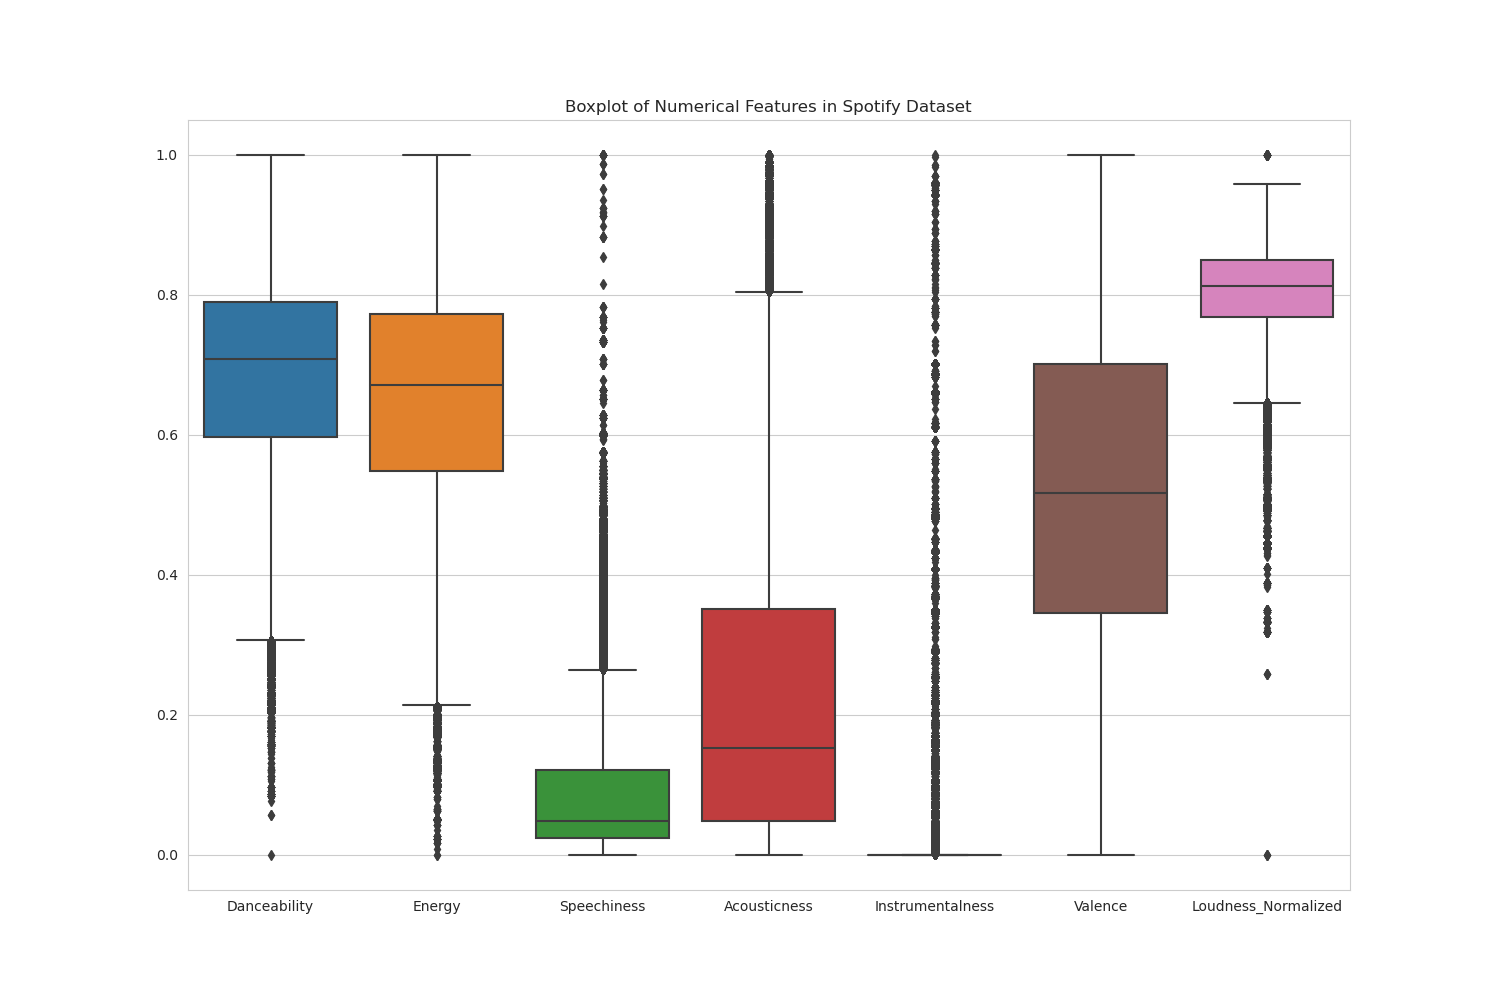
\includegraphics[width=0.8\textwidth]{boxplot.png}
  \captionsetup{labelformat=default}
  \caption{Box plot of Acoustic features}
  \label{fig:boxplot}
\end{figure}


\begin{figure}[h]
  \centering
  \includesvg[width=1\textwidth]{feature_trends}
  \captionsetup{labelformat=default}
  \caption{Normalized Trends of Acoustic Features Over time}
  \label{fig:feature_trends}
\end{figure}

\begin{figure}[h] % 可以使用figure环境来控制图片的浮动位置,选项[h]表示将图片放在当前位置
  \centering
  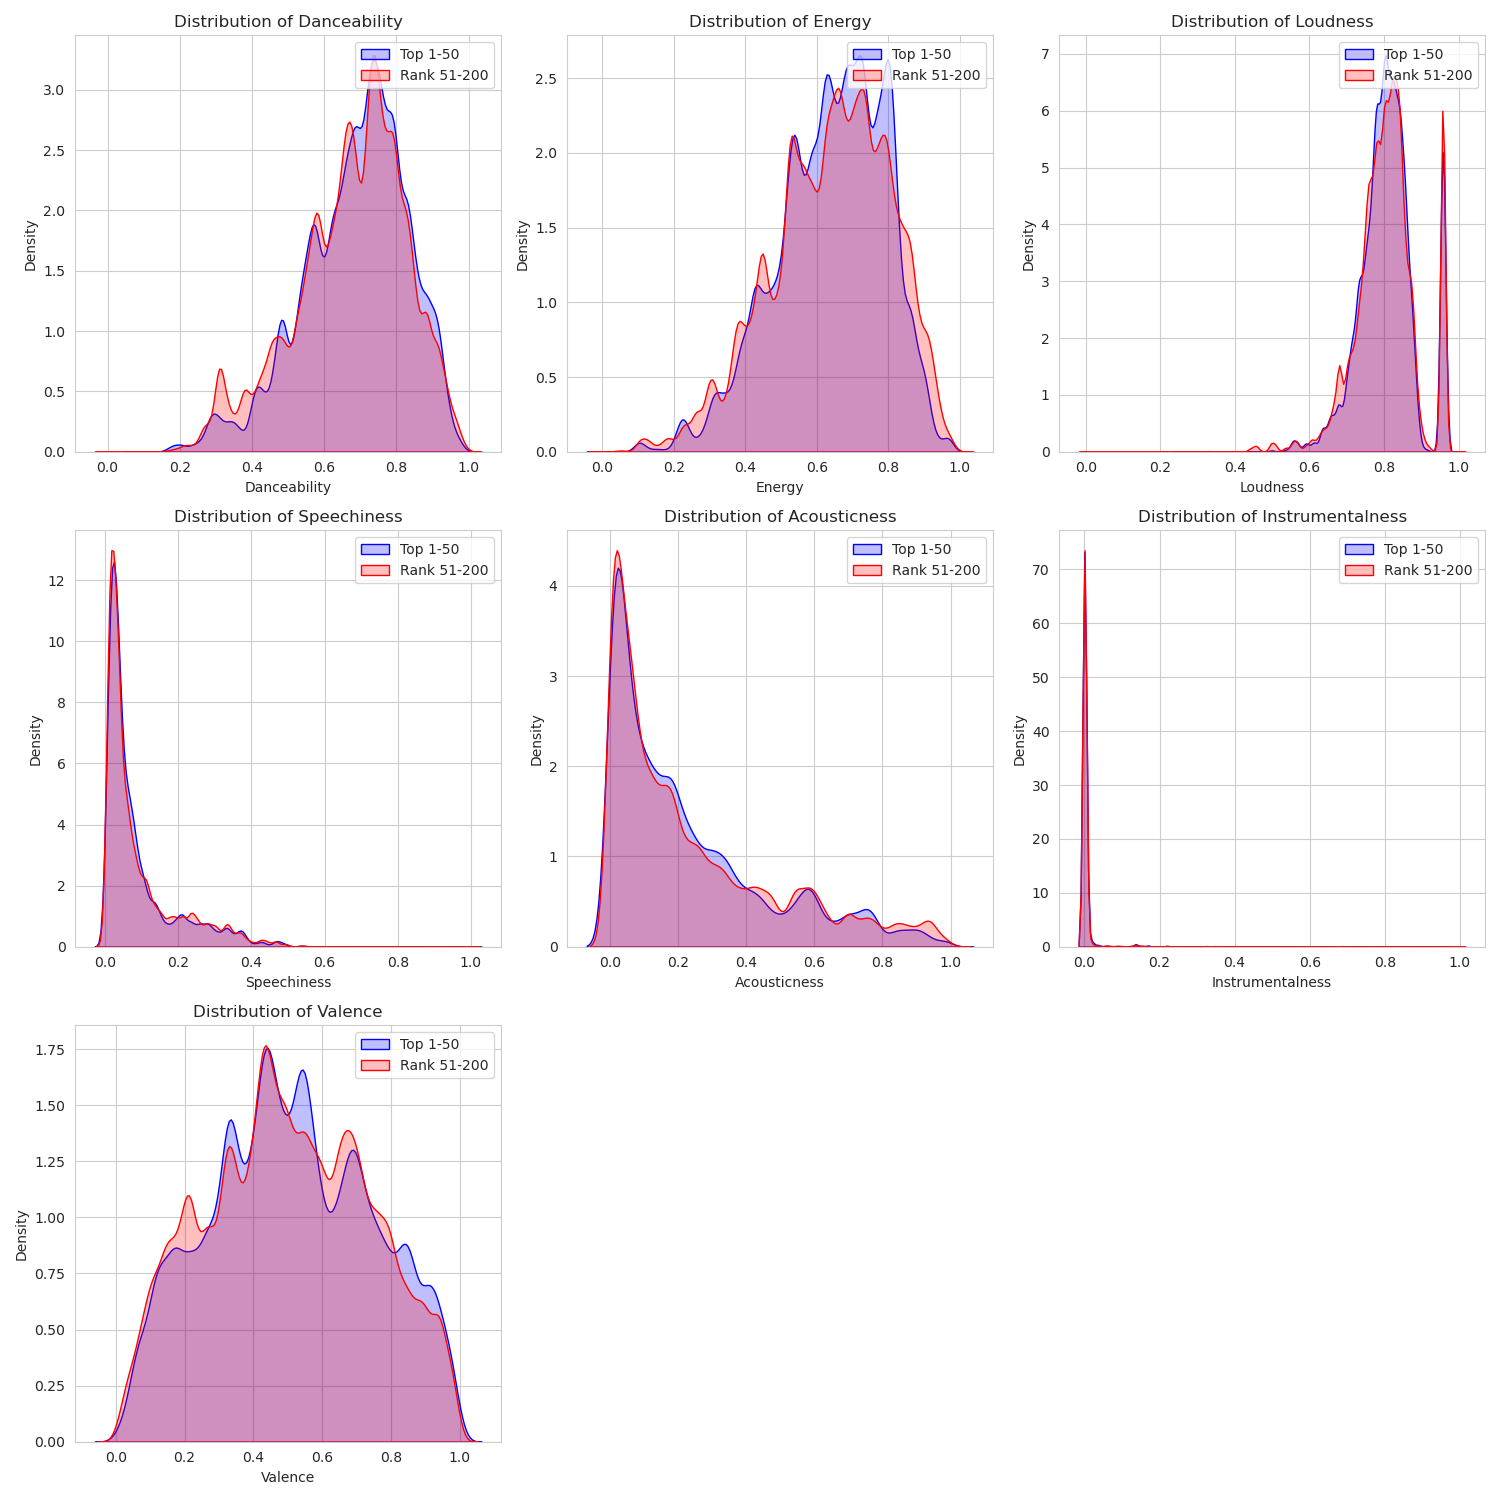
\includegraphics[width=0.8\textwidth]{distribute.png}
  \captionsetup{labelformat=default}
  \caption{Comparison of acoustic features distribution between Top50 and non Top50 songs. There is not a significant difference in the distribution of acoustic features between the top 50 and non top 50 songs.}
  \label{fig:distribute}
\end{figure}

\begin{figure}[h]
  \centering
  \includesvg[width=1\textwidth]{debut_new}
  \captionsetup{labelformat=default}
  \caption{Distribution of Song Debut Rankings}
  \label{fig:debut}
\end{figure}

\begin{figure}[h]
  \centering
  \includesvg[width=1\textwidth]{length}
  \caption{Normalized Distribution of Song Lengths in Top 50 Chart(2017-2022)}
  \label{fig:length}

  
\end{figure}

\end{document}




%%% Local Variables:
%%% mode: latex
%%% TeX-master: t
%%% End:
 